\chapter{Evaluation}

\section{Native vs Containerized vs Virtualized}

Der Performance-Test wird auf einer Node eines Compute-Clusters ausgeführt. Die Node hat folgende Spezifikationen:

\begin{itemize}
    \item CPU: AMD Epyc 7443, 2,85 GHz, 24 Core (48 Threads)
    \item RAM: 16 GB
    \item Speicher: NFS?
\end{itemize}

Für den Benchmark wird ein bereits existierendes Skript "benchmark.sh" verwendet, welches die Performance von allen möglichen Operationen, welche JULEA hat, getestet. Um das benchmark möglichst von externen Faktoren abhängig zu machen, wird der Benchmark auf einer Node eines Clusters als einziges Programm ausgeführt (exklusiv). Das benchmark wird 10-mal nacheinander ausgeführt, um die Konfidenz der Messergebnisse zu erhöhen (Vgl. \cite{kaliberaRigorousBenchmarkingReasonable2013} S. 11ff). 

\subsection{Native}

Die Messergebnisse des Benchmarks, welche Nativ auf dem Host-System ausgeführt wurden, lassen sich aus der folgenden Grafik entnehmen:

\begin{figure}[!h]
    \centering
    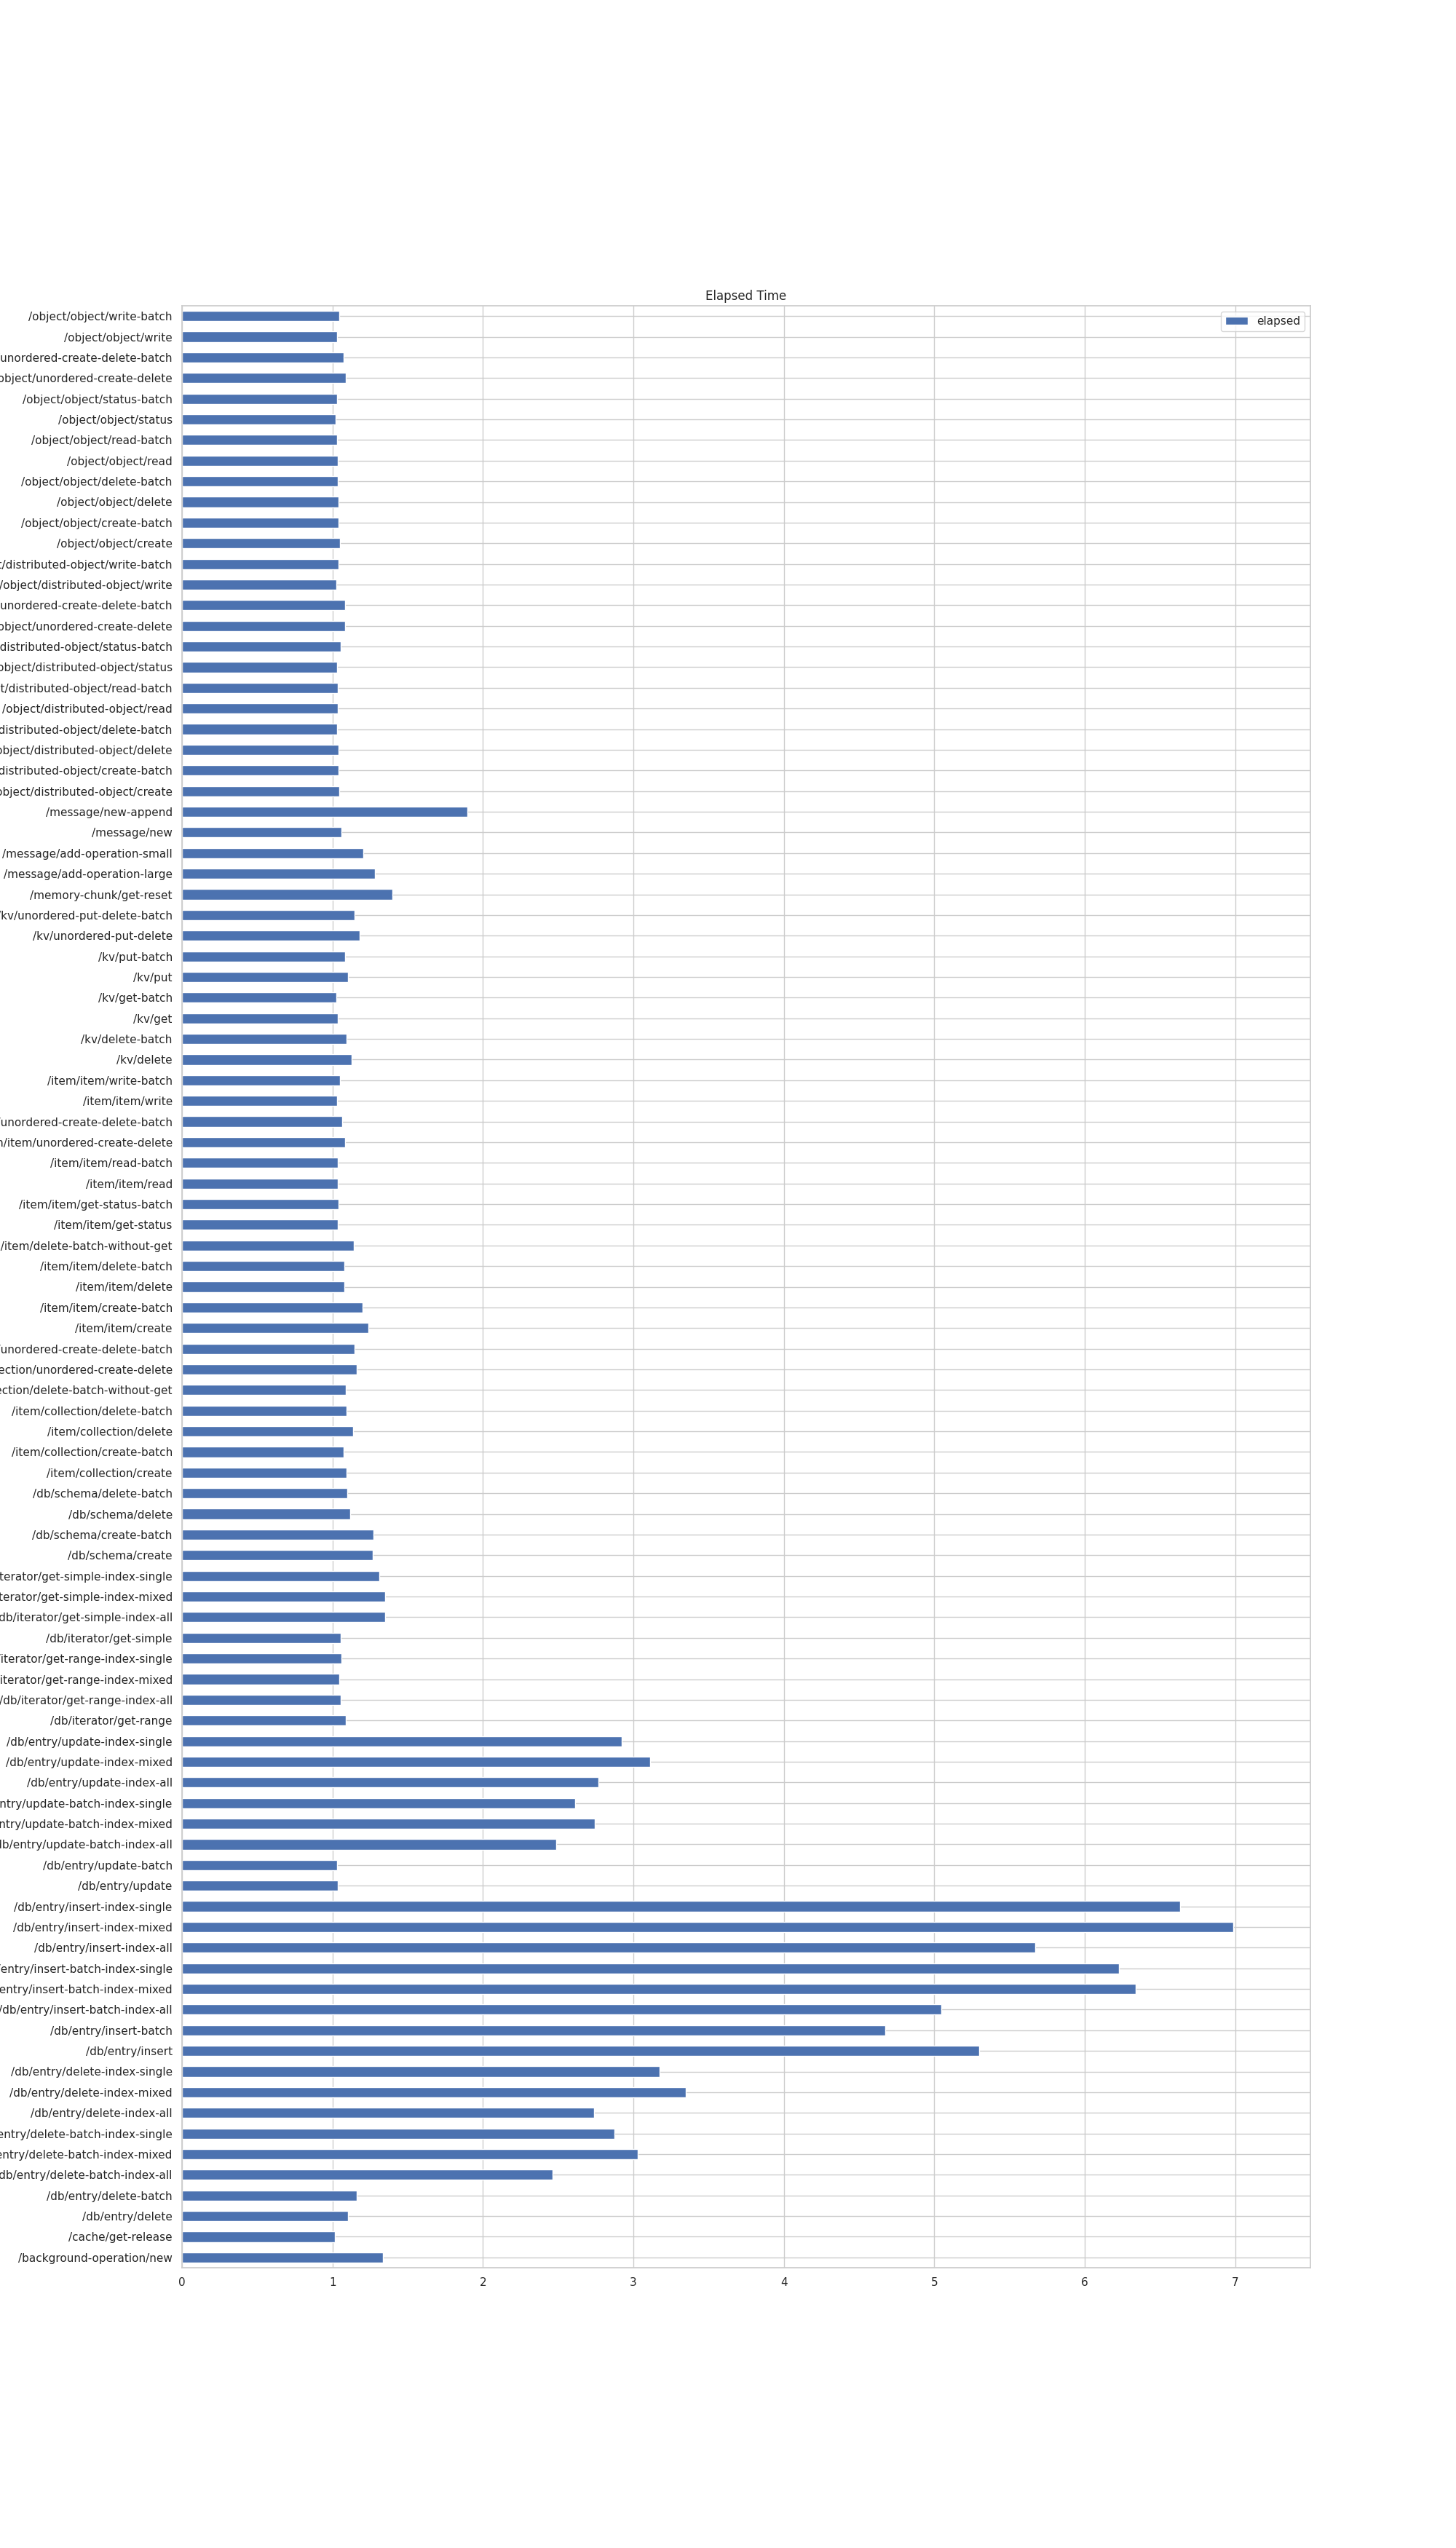
\includegraphics[width=0.8\textwidth]{benchmark/vis/system/elapsed.png}
    \caption{Performance-Test auf dem Host-System}
    \label{fig:native}
\end{figure}
\FloatBarrier

\subsection{Containerized}

Die Messergebnisse des Benchmarks, welche in einem Apptainer-Container ausgeführt wurden, lassen sich aus der folgenden Grafik entnehmen:

\begin{figure}[h!]
    \centering
    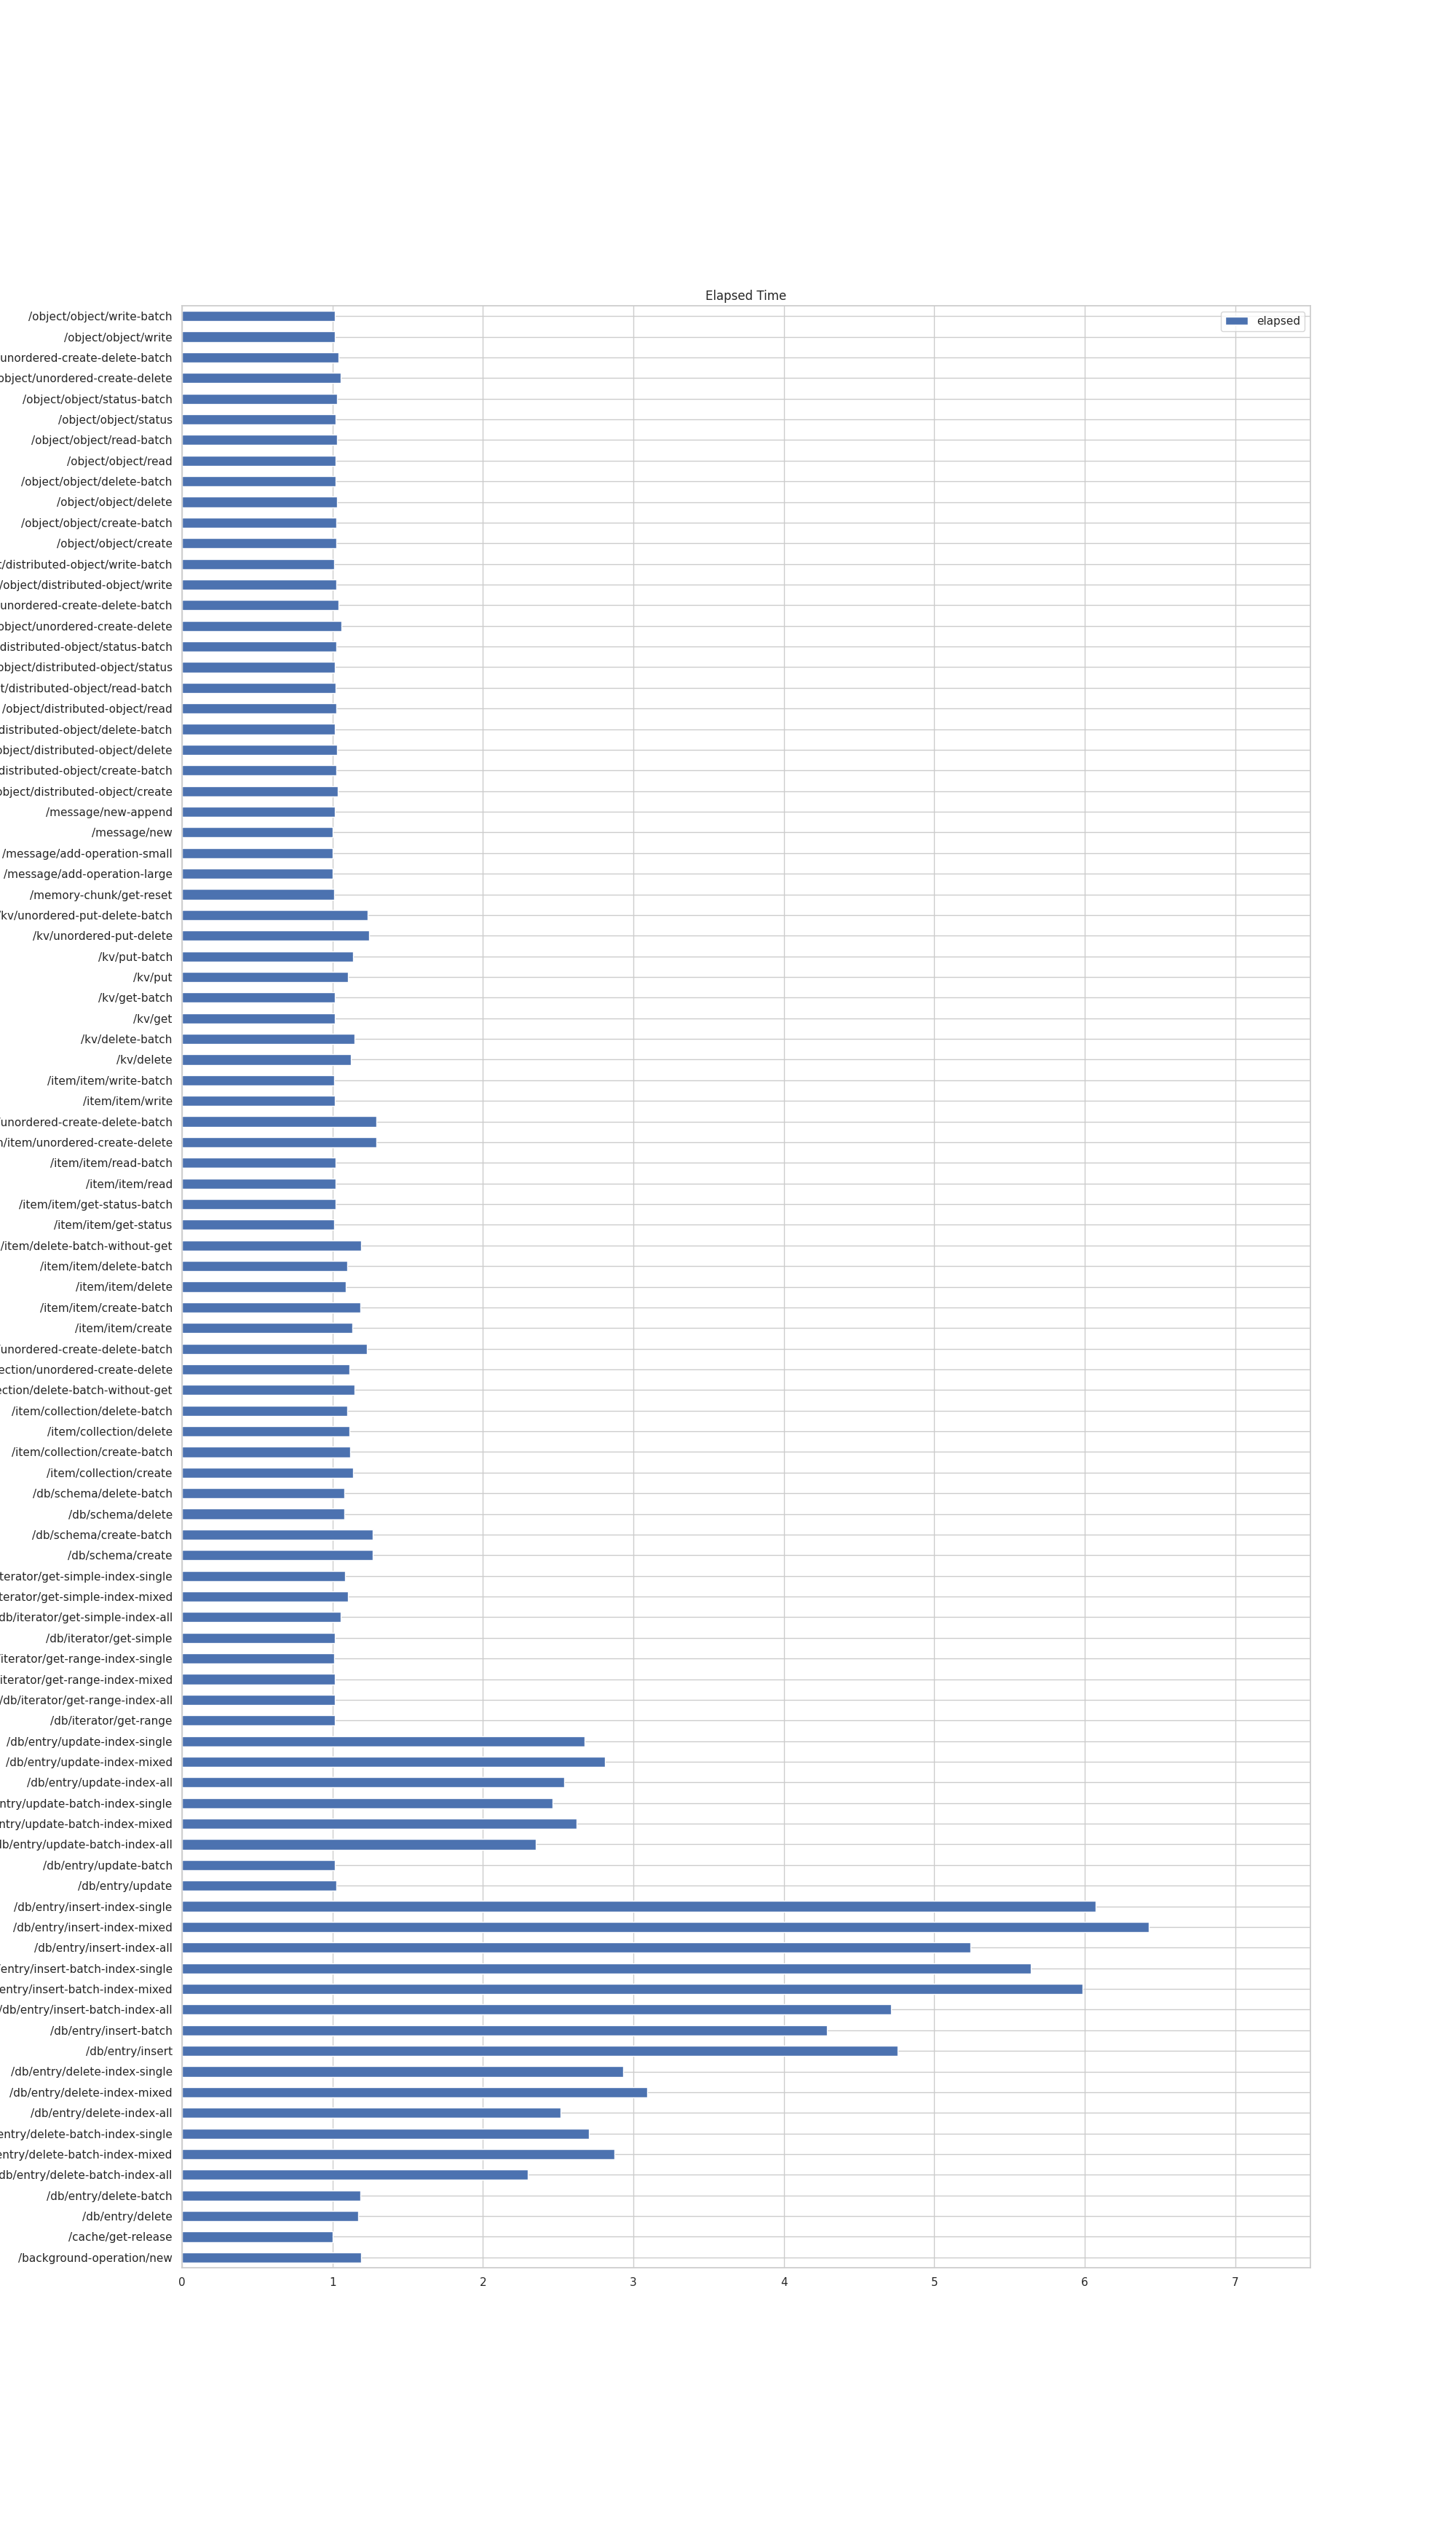
\includegraphics[width=0.8\textwidth]{benchmark/vis/apptainer/elapsed.png}
    \caption{Performance-Test in einem Apptainer-Container}
    \label{fig:apptainer}
\end{figure}
\FloatBarrier

\subsection{Virtualized}

\todo[inline]{Wie virtualisiert man auf dem Cluster?}

\subsection{Vergleich}

Die Performancedifferenz zwischen der Native- und Containerized-Ausführung des Benchmarks lässt sich aus der folgenden Grafik entnehmen. Ein negativer Wert bedeutet, dass die Containerized-Ausführung schneller war als die Native-Ausführung. Ein positiver Wert bedeutet, dass die Containerized-Ausführung langsamer war als die Native-Ausführung.

\begin{figure}[h!]
    \centering
    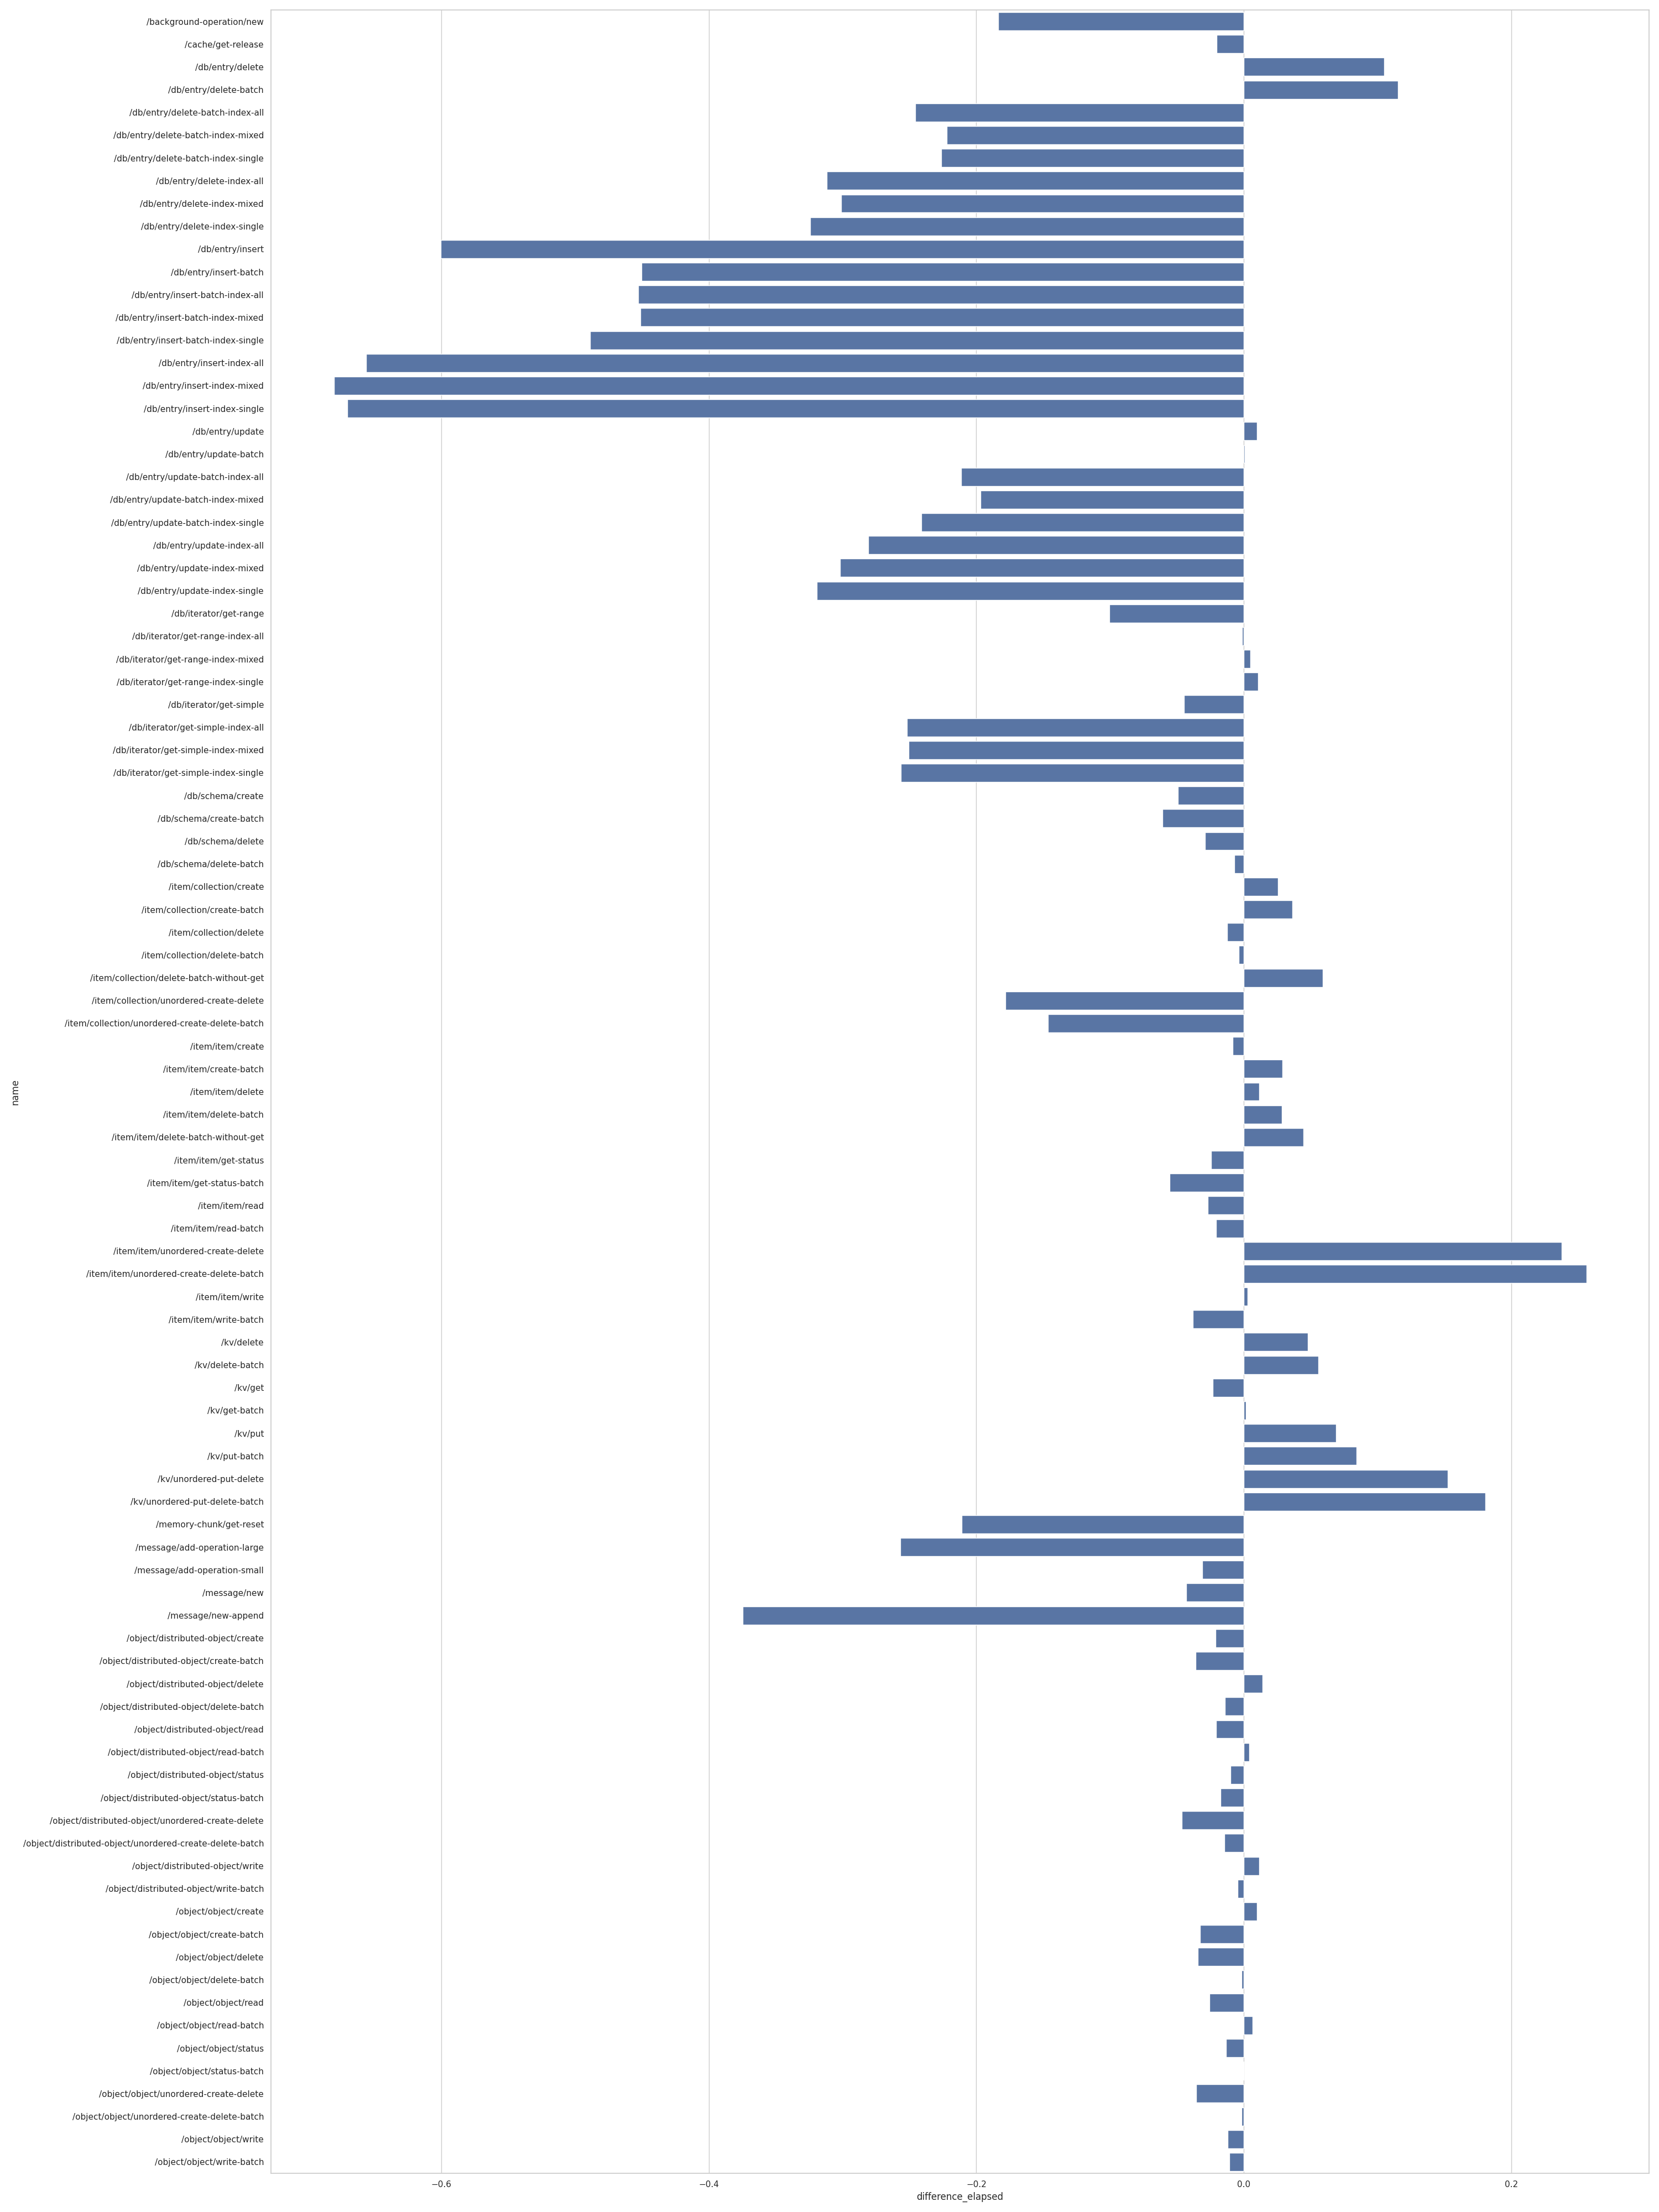
\includegraphics[width=0.8\textwidth]{benchmark/vis/differences/difference_elapsed.png}
    \caption{Vergleich der Performance}
    \label{fig:comparison}
\end{figure}

Aus der differenz der Messergebnisse lässt sich entnehmen, dass die Containerisierte Ausführung und die Native Ausführung des Benchmarks sich in der Performance nicht signifikant unterscheiden. 

\todo[inline]{Größe des Diagramms anpassen}
\FloatBarrier




